\documentclass[11pt]{article}
\usepackage[a4paper,margin=2.2cm]{geometry}
\usepackage[numbers,sort]{natbib}
\usepackage{amsmath,amssymb,booktabs,graphicx,xcolor,hyperref,multirow,caption,subcaption,enumitem,float}
\hypersetup{colorlinks=true,linkcolor=blue!50!black,citecolor=blue!50!black,urlcolor=blue!50!black}
\captionsetup{font=small,labelfont=bf}
\setlist{itemsep=2pt,topsep=3pt}
\newcommand{\rmpp}{\textsc{ReMasker++}}
\newcommand{\remasker}{\textsc{ReMasker}}
\newcommand{\sg}{\operatorname{sg}}
\newcommand{\best}[1]{\textbf{#1}}

\title{\rmpp: Missingness-Aligned Masked Autoencoding with\\ Learned Uncertainty for Tabular Data Imputation}
\author{MA 305: Data Science --- End-Term Project Report (Team 2)\\[4pt]
\small Jandhyala Mohana Sarath Chandra (240041020) \quad Aayush Sharma (240041001)\\ \small Arnav Nitin Birari (240041004)\\
\small Instructor: Prof.\ M.\ Tanveer\\ \small Code: \url{https://github.com/sunno-bhaato/remasker_pp}}
\date{November 18, 2026}

\sloppy
\begin{document}
\maketitle

\begin{abstract}
\rmpp{} improves on \remasker{} (ICLR 2024), a masked-autoencoder imputer for tabular data. It targets the limitations the \remasker{} authors themselves report. (i)~\emph{Missingness-aligned re-masking}: every training row is re-masked with the real missingness pattern of another row instead of a uniformly random mask, so the self-supervised task matches the test-time task. (ii)~A \emph{learned uncertainty head}, trained with stop-gradients on re-masked cells, predicts the expected error of every imputed cell without changing the imputations. (iii)~An optional exact 1-D \emph{Wasserstein objective} for distributional fidelity. On 5~datasets $\times$ MCAR/MAR/MNAR $\times$ 3~seeds, \rmpp{} reduces RMSE by 11.5\% and Wasserstein distance by 25\% relative to the official \remasker{}, and beats \remasker{} and MissForest in all 15 dataset--mechanism settings on both metrics. Against HyperImpute, the strongest baseline, \rmpp{} is competitive: it wins 6 of 15 settings on RMSE, and the (W) variant has the best average rank on WD and on downstream XGBoost utility. Under MNAR with 50--70\% missing values, \rmpp{} has the lowest RMSE of all methods. Its uncertainty estimates correlate with the true errors (Spearman $\rho=0.47$, versus $0.17$ for Monte-Carlo re-masking), and the 25\% most confident imputations are $3.5\times$ more accurate than the 25\% least confident ones. This enables selective imputation. A control experiment shows that about half of the RMSE gain comes from the structure of the copied masks rather than their lower masking ratio. We also report three components that did not help.
\end{abstract}

%======================================================================
\section{Introduction}
Missing values are ubiquitous in real-world tabular data, and most downstream learners require complete inputs, making \emph{imputation} a routine but consequential preprocessing step. \remasker{} \citep{du2024} (ICLR 2024) recast imputation as masked autoencoding: in addition to the naturally missing cells, a random subset of the \emph{observed} cells is ``re-masked'', a Transformer autoencoder is trained to reconstruct them, and the trained model is then applied to the truly missing cells. Despite its simplicity, \remasker{} matched or outperformed thirteen established imputers.

The authors themselves identify three limitations: (i) a growing gap between the distribution of re-masked cells (uniformly random) and of truly missing cells, which degrades performance from MCAR to MAR to MNAR; (ii) an MSE objective that favours point accuracy (RMSE) over distributional fidelity (Wasserstein distance, WD); and (iii) no mechanism to tell the user \emph{which} imputations can be trusted. Since 2024, several follow-ups have reported improvements over \remasker{}: CACTI \citep{cacti} (ICML 2025) with copy-masking and LLM-derived column context, PMAE \citep{pmae} with proportional masking, diffusion-based imputers such as DiffPuter \citep{diffputer} (ICLR 2025) and RefiDiff (AAAI 2026), and zero-shot foundation models such as TabImpute \citep{tabimpute}.

In this project we move beyond reproduction and \textbf{design, implement and rigorously evaluate an improved algorithm, \rmpp}, that targets each of these limitations. Our contributions are:
\begin{enumerate}
\item \textbf{Missingness-aligned re-masking.} During training, every row is re-masked with the \emph{real} missingness pattern of another row instead of a uniformly random mask, so that the self-supervised training task matches the test-time task.
\item \textbf{Learned per-cell uncertainty.} A lightweight heteroscedastic head, trained on \emph{stop-gradient} decoder features with a Gaussian negative log-likelihood, predicts the expected squared error of every imputed cell \emph{without changing the imputations}. This gives \rmpp{} a capability \remasker{} lacks: calibrated confidence and \emph{selective imputation}.
\item \textbf{Distribution-matching objective} (optional variant \rmpp{}\,(W)): an exact per-feature 1-D Wasserstein term that trades a little RMSE for better distributional fidelity.
\item \textbf{An efficient, equivalent re-implementation} of the \remasker{} architecture with attention key-padding masks, which batches inference (the official code imputes one row at a time) and removes a corner case where missing values were fed to the encoder as zeros.
\item \textbf{A systematic evaluation}: a full ablation of six candidate components (including three that \emph{did not} help, reported honestly), a benchmark against eight established imputers on five datasets, three missingness mechanisms and three seeds, downstream utility with two learners against a complete-data oracle, uncertainty calibration, and an MNAR stress test up to 70\% missingness.
\end{enumerate}

%======================================================================
\section{Background}
\paragraph{Missingness mechanisms.} Let $x\in\mathbb{R}^d$ be a record and $m\in\{0,1\}^d$ its observation mask. Data are \emph{MCAR} if $p(m\mid x)$ does not depend on $x$, \emph{MAR} if it depends only on the observed entries, and \emph{MNAR} otherwise (missingness depends on the missing values themselves) \citep{little}.

\paragraph{\remasker.} Values are min--max normalised and each feature is embedded by a shared linear map plus a fixed sinusoidal positional (feature-index) embedding. For each training row, the observed index set $O$ is split into a visible set $V$ and a re-masked set $R$ (uniformly at random, ratio $r=0.5$). The encoder (a Transformer) sees only the tokens in $V$; the decoder receives encoder outputs for $V$ and a shared learnable \texttt{[mask]} token elsewhere, and predicts every cell. The loss is
$\mathcal{L}_{\text{MSE}} = \tfrac{1}{|R|}\sum_{k\in R}(\hat x_k-x_k)^2 + \tfrac{1}{|V|}\sum_{k\in V}(\hat x_k-x_k)^2.$
At inference the encoder sees all observed cells and the decoder predicts the missing ones.

\paragraph{Related work since \remasker.} \textbf{CACTI} \citep{cacti} re-masks with observed missingness patterns (median-truncated copy masking) and adds LLM embeddings of column descriptions; \textbf{PMAE} \citep{pmae} masks features in proportion to their missing rate; \textbf{DiffPuter} \citep{diffputer} combines a diffusion model with EM; \textbf{TabImpute} \citep{tabimpute} is a pre-trained TabPFN-style transformer for zero-shot imputation. Classical strong baselines include \textbf{HyperImpute} \citep{hyperimpute} (an automatically configured column-wise ensemble, the strongest competitor in the \remasker{} paper), \textbf{MissForest}, \textbf{MICE}, \textbf{GAIN}, \textbf{MIWAE}, optimal-transport \textbf{Sinkhorn} imputation and \textbf{SoftImpute}.

%======================================================================
\section{Method: \rmpp}
Figure~\ref{fig:arch} summarises the design. \rmpp{} keeps \remasker's encoder--decoder exactly and changes (a) how training masks are generated, (b) what the model outputs and (c) the objective.

\begin{figure}[t]
\centering
\fbox{\begin{minipage}{0.95\linewidth}\small
\textbf{Training step (one mini-batch $B$)}\\[2pt]
1.\;For each row $i$ with observed set $O_i$: draw a donor row $j\in B$ and set $R_i = O_i\cap M_j$, $V_i = O_i\setminus M_j$ \hfill \emph{(missingness-aligned re-masking)}\\
\phantom{1.}\;\;if $R_i=\emptyset$ or $V_i=\emptyset$: fall back to a uniformly random split with ratio $0.5$.\\
2.\;$h=\text{Decoder}(\text{Encoder}(x_{V}),\,\texttt{[mask]}_{\bar V})$;\quad $\hat x=\tfrac12\tanh(w^\top h)+\tfrac12$;\quad $s=g_\phi(\sg(h))$ \hfill \emph{(uncertainty head)}\\
3.\;$\mathcal{L}=\mathcal{L}_{\text{MSE}}(\hat x)+\mathcal{L}_{\text{unc}}(s)\;[+\,\lambda\,\mathcal{L}_{W}(\hat x)]$\\[4pt]
\textbf{Imputation:} one batched pass with $V=O$; output $\hat x_k$ and confidence $\hat\sigma_k=e^{s_k/2}$ for each missing cell $k$.
\end{minipage}}
\caption{\rmpp{} at a glance. $M_j$ is the set of naturally missing features of the donor row; $\sg$ is stop-gradient.}
\label{fig:arch}
\end{figure}

\subsection{Missingness-aligned re-masking}
\remasker{} learns to reconstruct cells hidden by a \emph{uniform} mask, but at test time it must reconstruct cells hidden by the \emph{true} missingness mechanism, which is structured (e.g.\ under MAR/MNAR certain features are missing together, or only when other features take particular values). The authors attribute \remasker's degradation from MCAR to MNAR to exactly this mismatch. We close it by sampling training masks from the empirical distribution of missingness patterns: for row $i$ we copy the missing set $M_j$ of a random donor row $j$ in the mini-batch and hide $R_i=O_i\cap M_j$. Under MCAR and MAR, the resulting masks have the same joint structure (which features are missing together and how many) as the real ones; under MNAR the patterns are still realistic although the value-dependence cannot be reproduced. We apply copy-masking to every row ($p_{\text{copy}}=1$; $0.5$ is ablated), falling back to a uniform mask when the donor pattern is degenerate. The idea is related to CACTI's copy masking \citep{cacti}; differently from CACTI we use no external context (no LLM), keep \remasker's architecture and loss unchanged, and combine it with the uncertainty head below. Because copied masks hide fewer cells than \remasker's 50\% (roughly the dataset's missing rate), we additionally run a \textbf{control} with uniform masking at ratio $0.3$ to separate the effect of mask \emph{structure} from mask \emph{ratio}.

\subsection{Learned per-cell uncertainty with stop-gradient}
A point imputation hides how reliable it is. We attach a two-layer MLP $g_\phi$ to the \emph{detached} decoder features and train it on the re-masked cells with a Gaussian negative log-likelihood whose mean is also detached:
\[
\mathcal{L}_{\text{unc}}=\frac{1}{|R|}\sum_{k\in R}\Big[s_k+\big(x_k-\sg(\hat x_k)\big)^2 e^{-s_k}\Big],\qquad s_k=g_\phi(\sg(h_k)).
\]
For fixed $\hat x$, the minimiser is $e^{s_k}=\mathbb{E}\big[(x_k-\hat x_k)^2\mid\text{context}\big]$, so $\hat\sigma_k=e^{s_k/2}$ estimates the \emph{expected error of that specific imputation}. Because of the two stop-gradients, $\mathcal{L}_{\text{unc}}$ sends no gradient to the encoder, decoder or prediction head: the imputations are those of the model without the head (up to random-number-stream differences), so there is no accuracy--calibration trade-off. Supervision is available precisely because re-masked cells have known ground truth, and with missingness-aligned re-masking they mimic real missing cells.

\subsection{Distribution-matching objective (\rmpp{}\,(W))}
MSE regression shrinks predictions towards conditional means, compressing the imputed distribution and inflating WD (the authors note \remasker{} sometimes wins on RMSE but loses on WD). For each feature $j$, let $\hat x^{(j)}_{(1)}\le\dots\le\hat x^{(j)}_{(n_j)}$ and $x^{(j)}_{(1)}\le\dots\le x^{(j)}_{(n_j)}$ be the sorted predictions and ground truths of the re-masked cells of feature $j$ in the batch. Then
\[
\mathcal{L}_W=\frac{1}{|J|}\sum_{j\in J}\frac{1}{n_j}\sum_{i=1}^{n_j}\big(\hat x^{(j)}_{(i)}-x^{(j)}_{(i)}\big)^2
\]
is the exact squared 2-Wasserstein distance between the empirical marginals (the optimal 1-D coupling is the monotone one), differentiable and $O(n\log n)$. We use $\lambda=0.3$.

\subsection{Batched, equivalent architecture}
The official code removes non-visible tokens with \texttt{gather}, which requires the same number of visible tokens in every row of a batch; at inference it therefore processes one row at a time, and during training rows with fewer observed values than the keep budget feed their \emph{missing} cells (as zeros) to the encoder. We instead pass all tokens with an attention \emph{key-padding mask} over non-visible ones. Since padded keys receive zero attention weight and padded query outputs are replaced by \texttt{[mask]} tokens before decoding, this is the same function as token dropping, but it supports arbitrary per-row visibility, batched inference and copy-masking (whose masks have variable size).

\subsection{Components we tried that did not help}
For completeness we also implemented and ablated: \textbf{(B)} a missingness-pattern embedding (the row's natural mask, linearly embedded and added to the CLS and decoder tokens); \textbf{(E)} Monte-Carlo re-masking at inference (averaging $K=20$ passes that additionally hide 25\% of observed cells, with their spread as an uncertainty estimate); and \textbf{(F)} uncertainty-guided progressive imputation, which commits the most confident fraction of each row's missing cells in each of 4 rounds and uses them as context for the rest (in the spirit of MaskGIT's confidence-ordered decoding). Their results are reported in the ablation.

%======================================================================
\section{Experimental setup}
\paragraph{Datasets.} Five UCI datasets used in the \remasker{} paper, covering regression and classification: \textbf{yacht} ($308\times6$, regression), \textbf{airfoil} ($1503\times5$, regression), \textbf{compression} ($1030\times8$, regression), \textbf{raisin} ($900\times7$, binary) and \textbf{wine} quality ($1599\times11$, 6 classes). The target column is excluded from imputation and used only for downstream evaluation. (We also fixed a data-loading issue in the official loader, which reads the CSV index column as a feature.)

\paragraph{Missingness.} MCAR, MAR and MNAR (logistic self-masking model) at a 30\% rate, generated with the \texttt{hyperimpute} simulator used by the \remasker{} paper; three seeds (0, 1, 2) per setting, i.e.\ $5\times3\times3=45$ runs per method. MAR/MNAR masks only affect a subset of the columns, so the realised overall missing rate is lower than 30\%.

\paragraph{Baselines.} Official \remasker{} (unmodified model code, same training budget), HyperImpute, MissForest, MICE, GAIN, MIWAE, Sinkhorn, SoftImpute and Mean imputation (all from \texttt{hyperimpute}, default settings).

\paragraph{Metrics.} On min--max normalised data, over the artificially removed cells: \textbf{RMSE}, MAE and \textbf{WD} (the mean over features of the 1-D Wasserstein distance between imputed and true values). \textbf{Downstream utility}: 5-fold cross-validated XGBoost and linear models (logistic/ridge regression) trained on the imputed features; AUROC (macro one-vs-rest for wine) or $R^2$, compared with an \emph{oracle} trained on the complete data. \textbf{Uncertainty}: Spearman correlation between $\hat\sigma$ and absolute error, and RMSE of the 25\% most and least confident cells.

\paragraph{Training budget.} All neural variants use \remasker's configuration for small datasets (embedding 32, encoder depth 4, decoder depth 2, 4 heads, mask ratio 0.5, AdamW, lr $10^{-3}$ with warm-up and cosine decay, batch 64) and a common budget of $\min(600\text{ epochs}, 4000\text{ optimiser steps})$, run on a single CPU thread per job (Apple M3 Pro, 10 jobs in parallel).

%======================================================================
\section{Results}
\subsection{Main benchmark}
Table~\ref{tab:main} reports RMSE and WD averaged over the five datasets, and Table~\ref{tab:rank} summarises average ranks over the 15 dataset--mechanism settings together with downstream utility. Per-dataset results are in Appendix~\ref{app:perds}.

\begin{table}[h]
\centering\small\setlength{\tabcolsep}{3.5pt}
\resizebox{\linewidth}{!}{\begin{tabular}{lcccccc}
\toprule
Method & \multicolumn{3}{c}{RMSE $\downarrow$} & \multicolumn{3}{c}{WD $\downarrow$}\\
 & MCAR & MAR & MNAR & MCAR & MAR & MNAR\\
\midrule
\rmpp{} & \underline{0.1558{\scriptsize$\pm$0.0033}} & \underline{0.1531{\scriptsize$\pm$0.0099}} & \underline{0.1613{\scriptsize$\pm$0.0023}} & 0.0594{\scriptsize$\pm$0.0009} & 0.0582{\scriptsize$\pm$0.0053} & 0.0643{\scriptsize$\pm$0.0020}\\
\rmpp{} (W) & 0.1607{\scriptsize$\pm$0.0022} & 0.1604{\scriptsize$\pm$0.0111} & 0.1660{\scriptsize$\pm$0.0016} & \textbf{0.0510{\scriptsize$\pm$0.0010}} & \underline{0.0520{\scriptsize$\pm$0.0055}} & \underline{0.0568{\scriptsize$\pm$0.0012}}\\
\remasker{} (official) & 0.1712{\scriptsize$\pm$0.0030} & 0.1752{\scriptsize$\pm$0.0123} & 0.1778{\scriptsize$\pm$0.0052} & 0.0725{\scriptsize$\pm$0.0035} & 0.0875{\scriptsize$\pm$0.0045} & 0.0737{\scriptsize$\pm$0.0045}\\
\midrule
HyperImpute & \textbf{0.1512{\scriptsize$\pm$0.0028}} & \textbf{0.1379{\scriptsize$\pm$0.0045}} & \textbf{0.1569{\scriptsize$\pm$0.0008}} & 0.0554{\scriptsize$\pm$0.0010} & \textbf{0.0520{\scriptsize$\pm$0.0069}} & \textbf{0.0526{\scriptsize$\pm$0.0031}}\\
MissForest & 0.1680{\scriptsize$\pm$0.0006} & 0.1738{\scriptsize$\pm$0.0086} & 0.1716{\scriptsize$\pm$0.0019} & 0.0838{\scriptsize$\pm$0.0016} & 0.0936{\scriptsize$\pm$0.0076} & 0.0866{\scriptsize$\pm$0.0033}\\
MICE & 0.2375{\scriptsize$\pm$0.0018} & 0.2232{\scriptsize$\pm$0.0090} & 0.2448{\scriptsize$\pm$0.0034} & \underline{0.0546{\scriptsize$\pm$0.0006}} & 0.0522{\scriptsize$\pm$0.0035} & 0.0597{\scriptsize$\pm$0.0009}\\
GAIN & 0.2101{\scriptsize$\pm$0.0040} & 0.2055{\scriptsize$\pm$0.0054} & 0.2209{\scriptsize$\pm$0.0074} & 0.1104{\scriptsize$\pm$0.0083} & 0.1154{\scriptsize$\pm$0.0063} & 0.1168{\scriptsize$\pm$0.0045}\\
MIWAE & 0.2672{\scriptsize$\pm$0.0253} & 0.2812{\scriptsize$\pm$0.0028} & 0.2821{\scriptsize$\pm$0.0202} & 0.1174{\scriptsize$\pm$0.0188} & 0.1277{\scriptsize$\pm$0.0073} & 0.1290{\scriptsize$\pm$0.0206}\\
Sinkhorn & 0.2210{\scriptsize$\pm$0.0032} & 0.2367{\scriptsize$\pm$0.0110} & 0.2250{\scriptsize$\pm$0.0018} & 0.1260{\scriptsize$\pm$0.0009} & 0.1398{\scriptsize$\pm$0.0026} & 0.1299{\scriptsize$\pm$0.0013}\\
SoftImpute & 0.2632{\scriptsize$\pm$0.0023} & 0.2446{\scriptsize$\pm$0.0059} & 0.2675{\scriptsize$\pm$0.0080} & 0.0820{\scriptsize$\pm$0.0023} & 0.0980{\scriptsize$\pm$0.0081} & 0.1025{\scriptsize$\pm$0.0200}\\
Mean & 0.2178{\scriptsize$\pm$0.0002} & 0.2279{\scriptsize$\pm$0.0026} & 0.2269{\scriptsize$\pm$0.0026} & 0.1677{\scriptsize$\pm$0.0005} & 0.1741{\scriptsize$\pm$0.0023} & 0.1740{\scriptsize$\pm$0.0016}\\
\bottomrule
\end{tabular}
}
\caption{Imputation fidelity at 30\% missingness (average over 5 datasets; mean $\pm$ std over 3 seeds). \textbf{Best}, \underline{second best}.}
\label{tab:main}
\end{table}

\begin{table}[h]
\centering\small
\resizebox{\linewidth}{!}{\begin{tabular}{lcccc|cc}
\toprule
& \multicolumn{4}{c|}{Average rank (15 settings) $\downarrow$} & \multicolumn{2}{c}{Downstream gap to oracle $\uparrow$}\\
Method & RMSE & WD & XGB & Overall & XGBoost & Linear\\
\midrule
HyperImpute & \textbf{1.53} & 2.93 & 3.13 & \textbf{2.53} & \textbf{-0.203} & \textbf{-0.092}\\
\rmpp{} (W) & 3.20 & \textbf{1.93} & \textbf{2.73} & 2.62 & -0.207 & -0.101\\
\rmpp{} & 1.60 & 3.27 & 3.60 & 2.82 & -0.208 & -0.095\\
MissForest & 4.07 & 6.20 & 4.60 & 4.96 & -0.209 & -0.103\\
\remasker{} (official) & 4.60 & 5.40 & 5.87 & 5.29 & -0.221 & -0.105\\
MICE & 8.67 & 2.73 & 8.73 & 6.71 & -0.267 & -0.169\\
GAIN & 7.00 & 8.40 & 6.87 & 7.42 & -0.227 & -0.125\\
Sinkhorn & 7.73 & 8.87 & 7.60 & 8.07 & -0.228 & -0.133\\
Mean & 8.00 & 10.80 & 5.47 & 8.09 & -0.212 & -0.120\\
SoftImpute & 9.67 & 6.60 & 8.60 & 8.29 & -0.244 & -0.152\\
MIWAE & 9.93 & 8.87 & 8.80 & 9.20 & -0.245 & -0.176\\
\bottomrule
\end{tabular}
}
\caption{Left: average rank over the 15 dataset $\times$ mechanism settings (1 = best). Right: downstream score minus complete-data (oracle) score, averaged over datasets (AUROC for raisin/wine, $R^2$ for regression; closer to 0 is better).}
\label{tab:rank}
\end{table}

\paragraph{\rmpp{} vs.\ \remasker.} \rmpp{} is better than the official \remasker{} in \textbf{all 15 settings on both RMSE and WD}, with average reductions of \textbf{11.5\% (RMSE)} and \textbf{25.4\% (WD)}. Its average rank improves from 5.29 to 2.82. Per dataset, the RMSE reduction ranges from 6\% (yacht) to 20\% (raisin). \rmpp{}\,(W) reduces WD by 34.6\%.

\paragraph{\rmpp{} vs.\ the field.} \rmpp{} also beats MissForest in all 15 settings on RMSE and WD. HyperImpute is the strongest baseline, as in the \remasker{} paper. It keeps the best overall rank (2.53), followed closely by \rmpp{}\,(W) (2.62) and \rmpp{} (2.82); every other method is above 4.9. On RMSE the two are nearly tied (average rank 1.53 vs.\ 1.60). \rmpp{} wins 6 of 15 settings: all three mechanisms on wine, the dataset with the most features, two of three on yacht, and raisin-MCAR. HyperImpute wins on the low-dimensional regression datasets airfoil (5 features) and compression, where column-wise gradient-boosted models are hard to beat. On WD, \rmpp{}\,(W) has the \textbf{best average rank of all methods} (1.93). For context, the \remasker{} paper also reports \remasker{} losing to HyperImpute on some datasets, and \rmpp{} closes most of that gap.

\paragraph{Downstream utility.} Utility differences among the top methods are small: the XGBoost gaps to the oracle of HyperImpute, \rmpp{}, \rmpp{}\,(W) and MissForest lie within 0.006 of each other. \rmpp{}\,(W) has the best average XGBoost rank (2.73) and beats HyperImpute in 9 of 15 settings. Both \rmpp{} variants improve on official \remasker{} (gap $-0.207$ vs.\ $-0.221$). The large absolute gap ($\approx -0.2$) comes mostly from the regression datasets, where losing 30\% of a key predictor (e.g.\ the Froude number in yacht) caps the achievable $R^2$ for any imputer. A notable side-finding is that Mean imputation is a competitive input for XGBoost (rank 5.47) despite its poor fidelity, because tree ensembles can isolate the constant fill value. This supports the \remasker{} authors' remark that imputation quality and task utility are not the same thing.

\subsection{Ablation: what helps and why}
\begin{table}[h]
\centering\small
\resizebox{\linewidth}{!}{\begin{tabular}{lccccc}
\toprule
Variant & RMSE & WD & $\Delta$RMSE & $\Delta$WD & $\Delta$RMSE (MNAR)\\
\midrule
\remasker{} (official) & 0.1748 & 0.0779 & +0.0\% & +0.0\% & +0.0\%\\
\midrule
(A) batched re-implementation & 0.1761 & 0.0816 & -0.2\% & +0.0\% & -1.8\%\\
(A)+(B) pattern embedding & 0.2072 & 0.0899 & +17.7\% & +20.9\% & +17.0\%\\
(A)+(D) Wasserstein loss, $\lambda{=}1$ & 0.1908 & 0.0694 & +7.4\% & -13.3\% & +4.5\%\\
(A)+(E) MC re-masking inference & 0.1660 & 0.0823 & -6.1\% & +1.7\% & -6.5\%\\
(A)+(E)+(F) progressive inference & 0.1739 & 0.0912 & -1.9\% & +12.4\% & +0.5\%\\
\midrule
(A) + uniform mask ratio 0.3 \emph{(control)} & 0.1679 & 0.0530 & -6.3\% & -32.8\% & -3.9\%\\
(A)+(C) copy-masking, $p_{\text{copy}}{=}0.5$ & 0.1593 & 0.0655 & -10.0\% & -20.2\% & -9.2\%\\
\midrule
\textbf{\rmpp}: (A)+(C, $p_{\text{copy}}{=}1$)+(G) & 0.1567 & 0.0607 & -11.5\% & -25.4\% & -9.7\%\\
\rmpp{} + (E) MC inference & 0.1602 & 0.0791 & -9.3\% & -2.2\% & -9.0\%\\
\rmpp{} + (F) progressive & 0.1639 & 0.0611 & -8.0\% & -23.9\% & -4.5\%\\
\textbf{\rmpp{}\,(W)}: \rmpp{} + (D), $\lambda{=}0.3$ & 0.1624 & 0.0533 & -8.8\% & -34.6\% & -7.3\%\\
\bottomrule
\end{tabular}
}
\caption{Ablation (average over 5 datasets $\times$ 3 mechanisms $\times$ 3 seeds). $\Delta$ = mean per-setting relative change vs.\ official \remasker{} (negative is better). Letters refer to Section~3.}
\label{tab:abl}
\end{table}

\begin{figure}[h]
\centering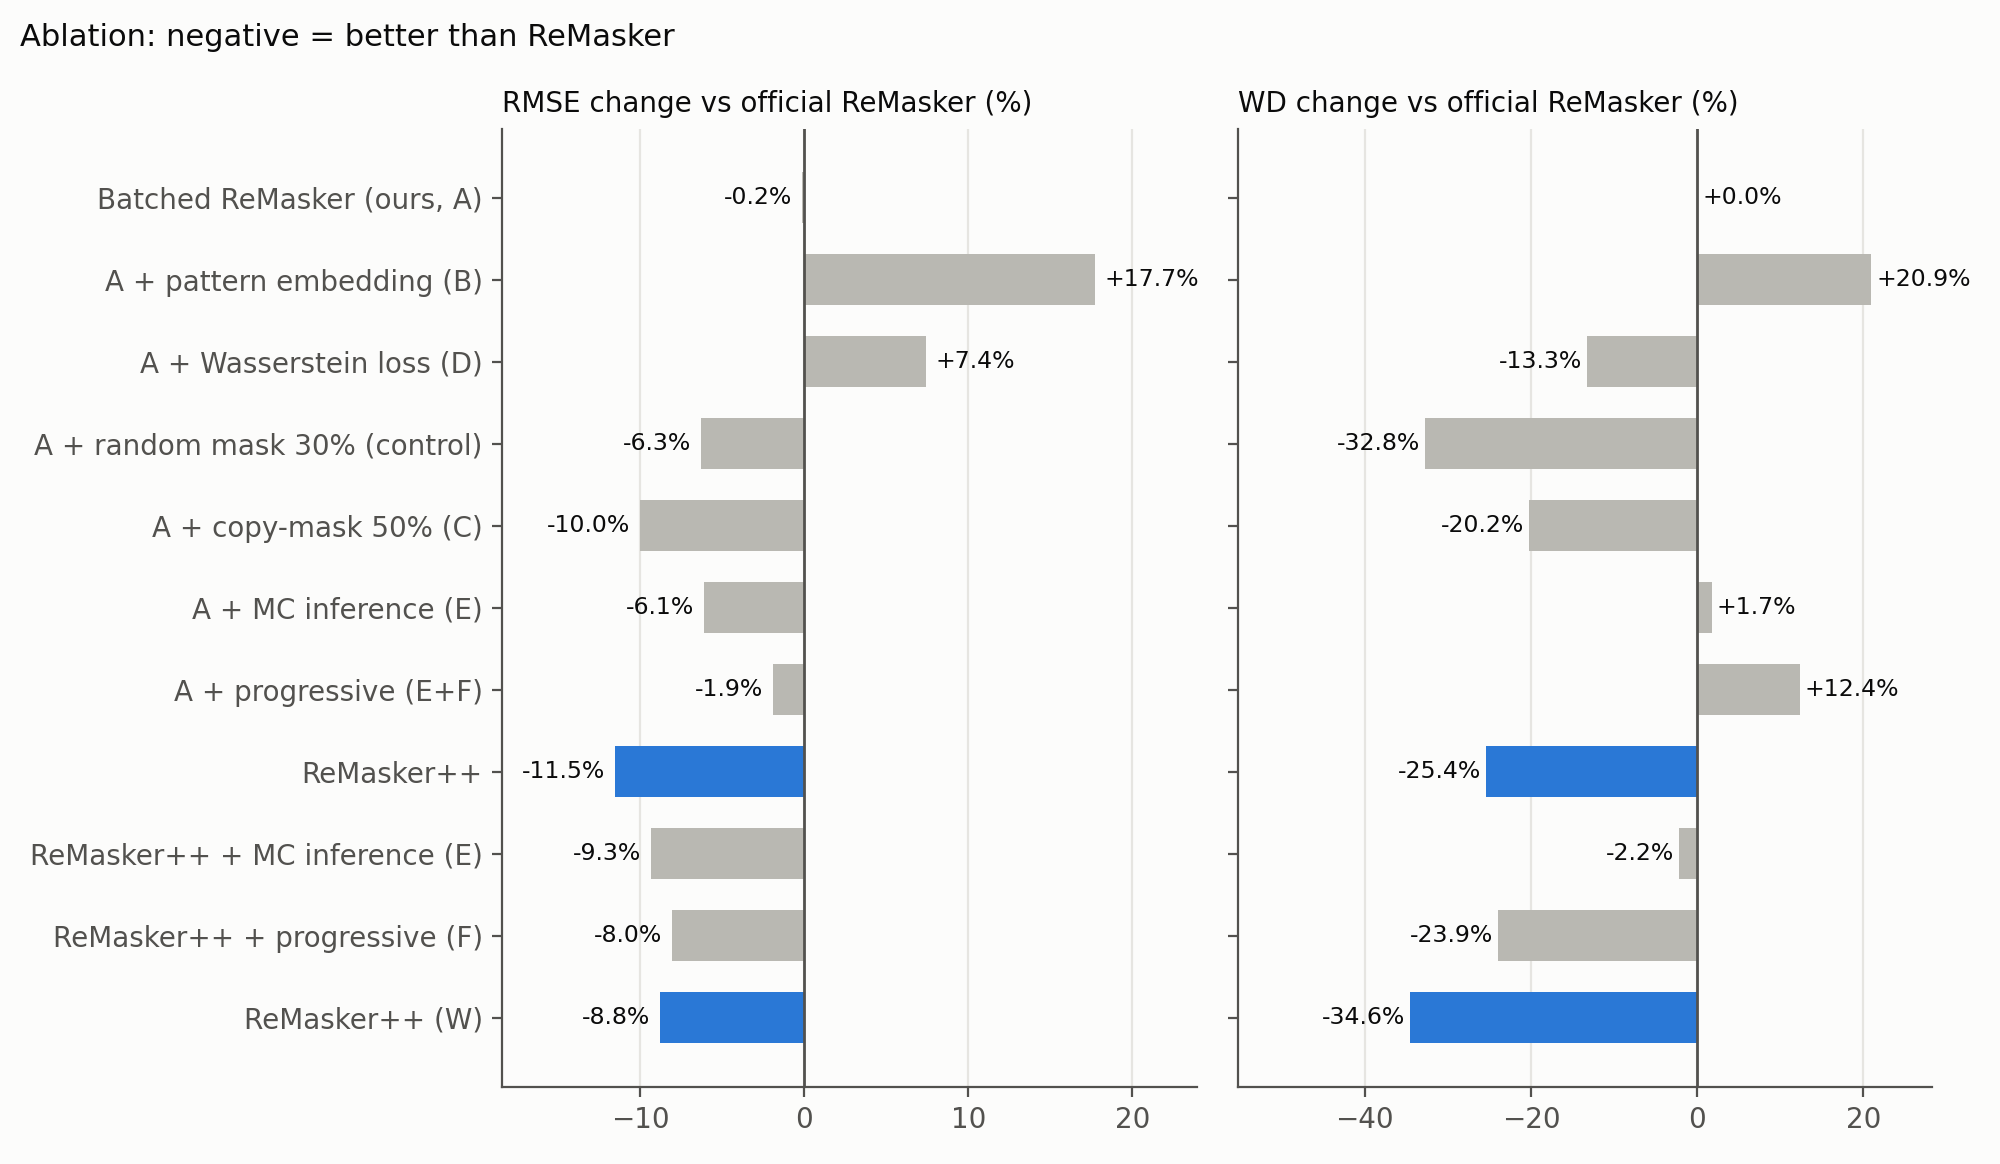
\includegraphics[width=0.95\linewidth]{../results/figures/ablation.png}
\caption{Ablation: relative change in RMSE and WD vs.\ official \remasker{} (negative is better).}
\label{fig:abl}
\end{figure}

Table~\ref{tab:abl} and Figure~\ref{fig:abl} isolate each component:
\begin{itemize}
\item \textbf{(A) Re-implementation is faithful:} $-0.2\%$ RMSE and $+0.0\%$ WD vs.\ the official code. The gains below therefore come from the method, not from implementation differences. Batched inference is $6\times$ faster than the official row-by-row inference (wine, 1599 rows: 1.46\,s vs.\ 0.23\,s).
\item \textbf{(C) Missingness-aligned re-masking is the main driver:} $-10.0\%$ RMSE with $p_{\text{copy}}=0.5$ and $-11.5\%$ with $p_{\text{copy}}=1$ (\rmpp), with the largest gains on MAR/MNAR.
\item \textbf{Control (structure vs.\ ratio):} copied masks hide fewer cells than \remasker's 50\%. Uniform masking at the matched ratio of 0.3 gives $-6.3\%$ RMSE, about half of \rmpp's gain. Under MNAR it gives only $-3.9\%$ vs.\ $-9.7\%$. So the lower ratio accounts for part of the improvement, and the \emph{structure} of realistic masks accounts for the rest, especially under MNAR. Interestingly, the control has the best WD of the ratio/structure variants: hiding fewer cells per row gives the decoder more context and yields less shrunken predictions. Also, the 0.5 masking ratio recommended in the \remasker{} paper is not optimal at 30\% missingness in our setting.
\item \textbf{(D) Wasserstein loss} behaves as designed: alone it reduces WD by 13\% but increases RMSE by 7\%. Combined with (C) at $\lambda=0.3$, it gives the best WD overall ($-34.6\%$) at a modest RMSE cost relative to \rmpp.
\item \textbf{(B) Pattern embedding hurts} ($+17.7\%$ RMSE). Adding a row-level missingness code to every decoder token lets the model fit pattern-specific shortcuts on these small datasets.
\item \textbf{(E) MC inference} helps the base model ($-6.1\%$ RMSE, an ensembling effect) but not \rmpp{}, and it increases WD (averaging shrinks predictions). \textbf{(F) Progressive imputation} is worse than one-shot imputation in every configuration. Committed imputations are smoother than real values, so later rounds condition on inputs unlike anything seen in training (exposure bias), and errors compound. This also holds when the ordering uses the well-calibrated learned uncertainty, so the problem is the conditioning, not the ordering signal.
\end{itemize}

\subsection{Uncertainty quality and selective imputation}
\begin{table}[h]
\centering\small
\resizebox{\linewidth}{!}{\begin{tabular}{lcccc}
\toprule
Uncertainty estimate & Spearman $\rho$ $\uparrow$ & RMSE, 25\% most confident & RMSE, 25\% least confident & ratio\\
\midrule
MC re-masking (E), base model & 0.171 & 0.1624 & 0.1754 & 1.08$\times$\\
MC re-masking (E), \rmpp & 0.188 & 0.1564 & 0.1707 & 1.09$\times$\\
\textbf{Learned head (G), \rmpp} & 0.470 & 0.0668 & 0.2316 & 3.47$\times$\\
Learned head (G), \rmpp{}\,(W) & 0.476 & 0.0714 & 0.2355 & 3.30$\times$\\
\bottomrule
\end{tabular}
}
\caption{Quality of per-cell uncertainty estimates (average over all 45 runs). Spearman correlation between predicted uncertainty and absolute error of the imputed cells; RMSE of the 25\% most and least confident cells.}
\label{tab:unc}
\end{table}

\begin{figure}[h]
\centering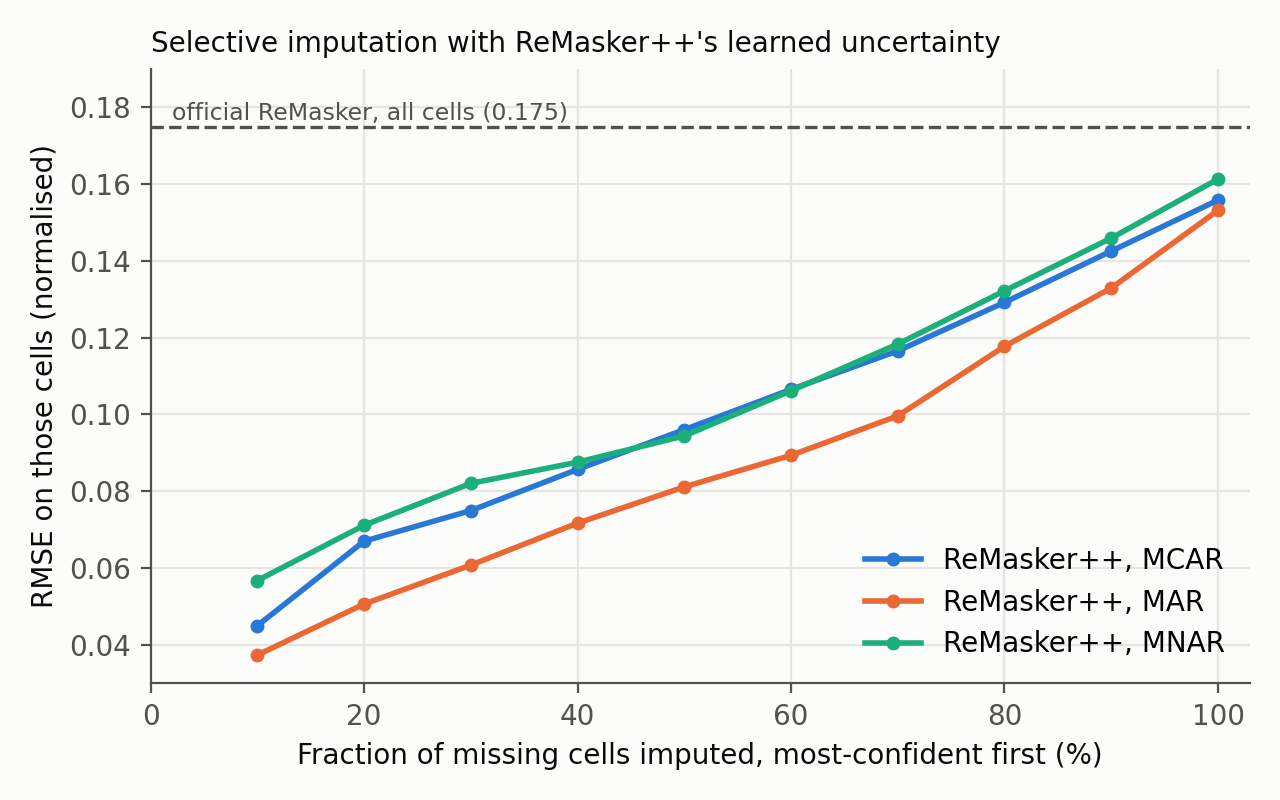
\includegraphics[width=0.62\linewidth]{../results/figures/coverage_curve.png}
\caption{Selective imputation: RMSE of the $c\%$ most confident imputed cells, as ranked by \rmpp's learned uncertainty, averaged over datasets and seeds. The dashed line is the RMSE of official \remasker{} on all cells.}
\label{fig:cov}
\end{figure}

The learned head produces informative uncertainty (Table~\ref{tab:unc}). Its Spearman correlation with the actual error is \textbf{0.47} (0.45 MAR, 0.46 MCAR, 0.50 MNAR), versus 0.17--0.19 for Monte-Carlo re-masking. The 25\% most confident cells have RMSE 0.067, against 0.232 for the 25\% least confident: a \textbf{3.5$\times$} separation. Figure~\ref{fig:cov} shows what this enables in practice. A practitioner can accept the most confident half of the imputations at roughly 40\% lower RMSE than the full set (about 0.09 vs.\ 0.155), and flag the rest for review or for multiple imputation. Even with all cells imputed, \rmpp's RMSE is below that of the official \remasker. As designed, adding the head does not degrade the imputations (Table~\ref{tab:abl}). Neither \remasker{} nor the other masked-autoencoder imputers provide this capability.

\subsection{Stress test: MNAR with heavy missingness}
\begin{figure}[h]
\centering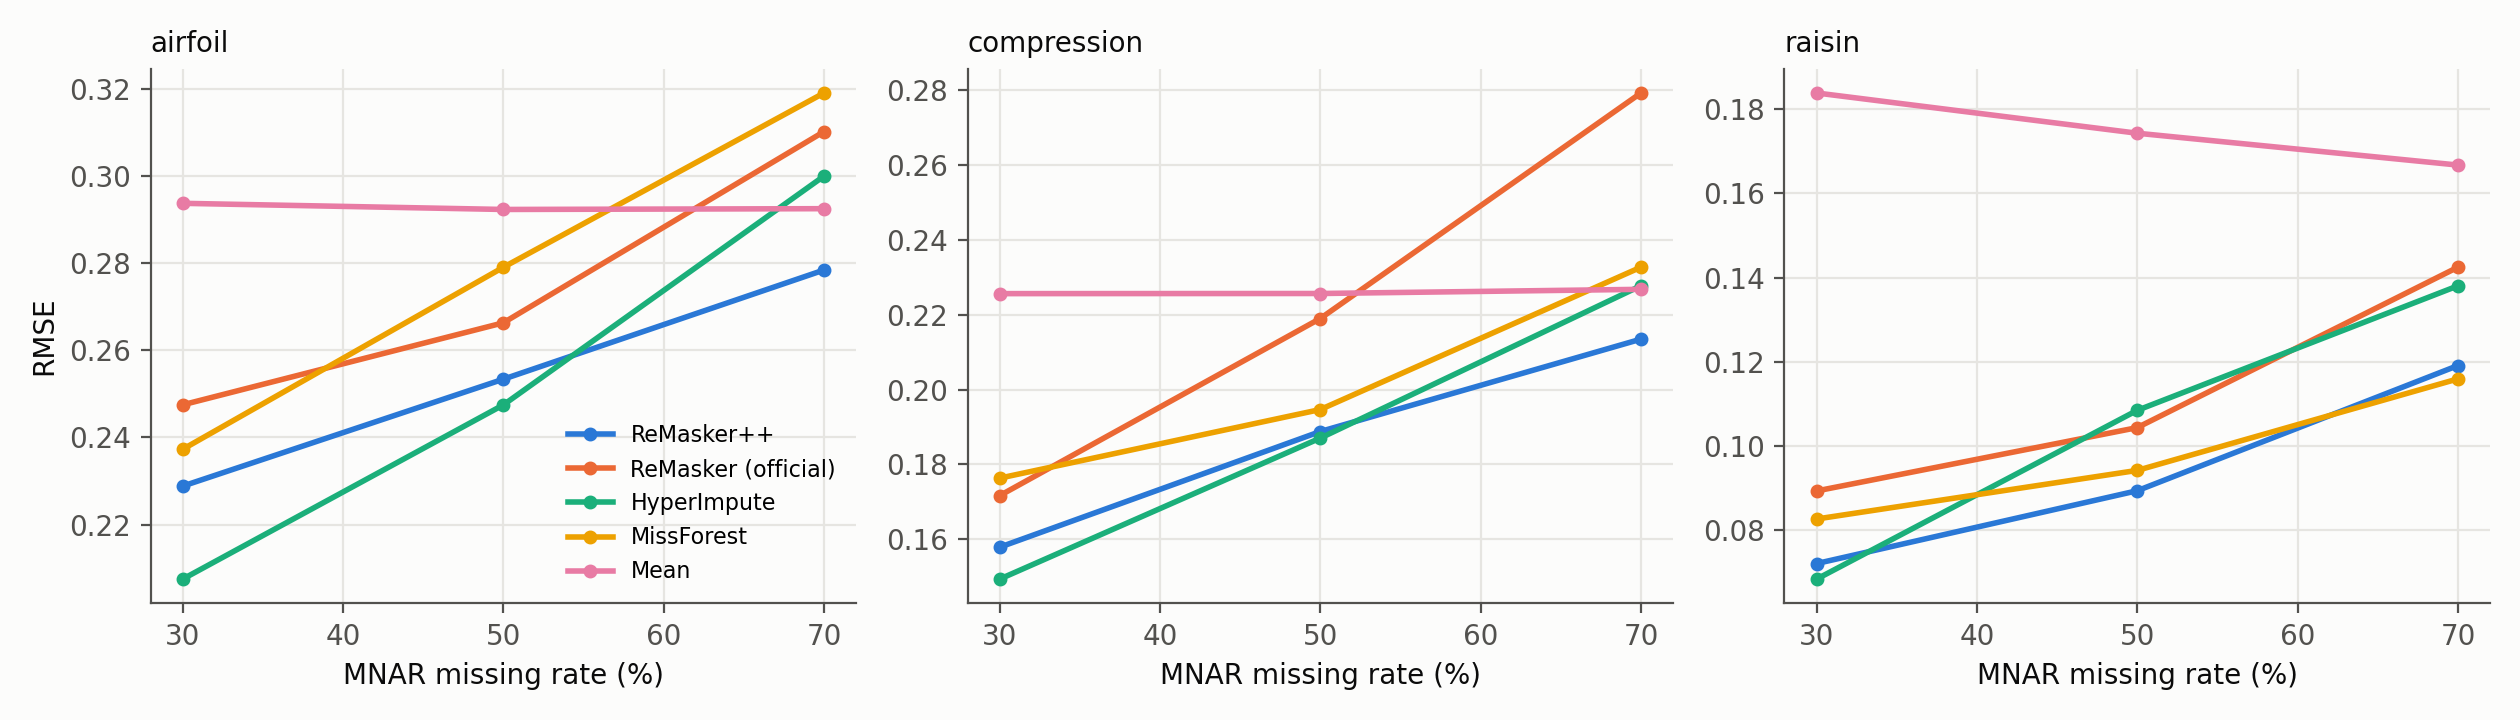
\includegraphics[width=\linewidth]{../results/figures/stress_mnar.png}
\caption{RMSE under MNAR as the missing rate grows from 30\% to 70\% (mean over 2 seeds).}
\label{fig:stress}
\end{figure}
\begin{table}[h]
\centering\small
\begin{tabular}{lccc}
\toprule
Method & 30\% & 50\% & 70\%\\
\midrule
\rmpp{} & 0.1529 & \textbf{0.1772} & \textbf{0.2037}\\
\remasker{} (official) & 0.1695 & 0.1966 & 0.2440\\
HyperImpute & \textbf{0.1418} & 0.1810 & 0.2220\\
MissForest & 0.1654 & 0.1893 & 0.2226\\
Mean & 0.2344 & 0.2308 & 0.2287\\
\bottomrule
\end{tabular}

\caption{MNAR stress test, RMSE averaged over airfoil, compression and raisin (2 seeds).}
\label{tab:stress}
\end{table}

MNAR is the hardest setting and the one where \remasker's authors report the largest degradation. Figure~\ref{fig:stress} and Table~\ref{tab:stress} push it to 50\% and 70\% missing values. The official \remasker{} degrades fastest (RMSE $0.170\to0.244$), and at 70\% it is worse than mean imputation on compression. \rmpp{} degrades most gracefully. HyperImpute is best at 30\%, but \rmpp{} has the \textbf{lowest average RMSE of all methods at 50\% and 70\%}. At 70\% it is 8\% better than HyperImpute and 17\% better than \remasker, and it beats HyperImpute on airfoil and compression. Its advantage over HyperImpute appears exactly where data are scarcest and missingness is most informative. Under those conditions, training on realistic missingness patterns matters most, and column-wise iterative methods lose the conditioning information they rely on.

%======================================================================
\section{Discussion}
\paragraph{Why missingness-aligned re-masking works.} Masked-autoencoder imputation trains on a proxy task: reconstructing cells \emph{we} hid. That proxy is only as good as its resemblance to the real task: reconstructing cells \emph{the world} hid. Uniform masking hides independent random cells at a fixed high rate. Real missingness is correlated across features, varies in amount between rows, and under MAR/MNAR depends on the data. Copying real patterns makes the proxy task match the real one in structure and in amount. Our control experiment separates these two effects: both matter, and structure matters most under MNAR.

\paragraph{Why the uncertainty head works and MC re-masking does not.} MC re-masking measures how much a prediction \emph{changes} when context is removed. That is a sensitivity measure, and for a well-trained deterministic network it is only weakly related to the error. The learned head is \emph{directly supervised} with the squared errors of re-masked cells, whose ground truth is known. Missingness-aligned masking makes these cells statistically similar to the truly missing ones, so the error predictor transfers to test-time imputations. The stop-gradients keep the two objectives from competing.

\paragraph{Positioning.} \rmpp{} is not a new state of the art over every method. HyperImpute, an automatically tuned ensemble of column-wise learners, still has the best overall rank in our benchmark. We did not re-run the 2025--26 methods (CACTI, DiffPuter, RefiDiff, TabImpute), which report gains over \remasker{} on their own benchmarks. What \rmpp{} shows is that a \emph{single} masked autoencoder, changed only in how it is trained, goes from mid-table (rank 5.3) to level with the best ensemble (rank 2.6--2.8). It gives the best distributional fidelity, is the most robust under heavy MNAR missingness, and is the only method in the comparison that reports how much each imputation can be trusted.

\paragraph{Limitations.} (1) Compute: models were trained under a 4000-step budget on CPU, with three seeds and five small-to-medium datasets; larger datasets (letter, spam) and full 600-epoch training were out of scope in the time available. (2) We did not re-run CACTI, DiffPuter or TabImpute ourselves; we position our work relative to their published claims and do not claim state of the art over them. (3) Like \remasker, \rmpp{} handles numerical (or ordinally encoded) features only. (4) Under MNAR, copied patterns reproduce the \emph{structure} but not the value-dependence of missingness.

\section{Conclusion and future work}
We extended \remasker{} into \rmpp{} by aligning its self-supervised training masks with the real missingness distribution, adding a stop-gradient uncertainty head, and optionally adding an exact Wasserstein objective. In a benchmark with 9 baselines, 5 datasets, 3 mechanisms, 3 seeds and a full ablation, \rmpp{} improves on \remasker{} in every setting ($-11.5\%$ RMSE, $-25\%$ WD) and is competitive with HyperImpute. It has the best WD and downstream ranks with the (W) variant, and the lowest error under heavy MNAR missingness. It also gives calibrated per-cell confidence, which supports selective imputation. Three plausible ideas (pattern embedding, MC inference and progressive imputation) did not help, and the reasons are informative in themselves.

\textbf{Future work:} (1) use the predicted uncertainty for \emph{multiple imputation} and propagate it into downstream models (e.g.\ Rubin's rules or uncertainty-weighted training); (2) learn the masking distribution (e.g.\ adversarially) instead of copying it, to also capture MNAR value-dependence; (3) categorical features via embeddings and a mixed loss; (4) head-to-head comparison with CACTI, DiffPuter and TabImpute on larger datasets with GPU-scale training; (5) an adaptive masking ratio tied to the observed missing rate, which our control suggests is beneficial.

\begin{thebibliography}{9}\small
\bibitem[Du et~al.(2024)]{du2024} T.~Du, L.~Melis, T.~Wang. ReMasker: Imputing tabular data with masked autoencoding. \emph{ICLR}, 2024.
\bibitem[Gorla et~al.(2025)]{cacti} A.~Gorla et~al. CACTI: Leveraging copy masking and contextual information to improve tabular data imputation. \emph{ICML}, PMLR 267, 2025.
\bibitem[PMAE(2024)]{pmae} To predict or not to predict? Proportionally masked autoencoders for tabular data imputation. arXiv:2412.19152, 2024.
\bibitem[Zhang et~al.(2025)]{diffputer} H.~Zhang et~al. DiffPuter: Empowering diffusion models for missing data imputation. \emph{ICLR}, 2025.
\bibitem[TabImpute(2025)]{tabimpute} TabImpute: Accurate and fast zero-shot missing-data imputation with a pre-trained transformer. arXiv:2510.02625, 2025.
\bibitem[Jarrett et~al.(2022)]{hyperimpute} D.~Jarrett et~al. HyperImpute: Generalized iterative imputation with automatic model selection. \emph{ICML}, 2022.
\bibitem[Little \& Rubin(2019)]{little} R.~Little, D.~Rubin. \emph{Statistical Analysis with Missing Data}. Wiley, 3rd ed., 2019.
\bibitem[Chang et~al.(2022)]{maskgit} H.~Chang et~al. MaskGIT: Masked generative image transformer. \emph{CVPR}, 2022.
\end{thebibliography}

\appendix
\section{Per-dataset RMSE}\label{app:perds}
\begin{table}[h]
\centering\setlength{\tabcolsep}{2.5pt}
\resizebox{\linewidth}{!}{\begin{tabular}{lccccccccccccccc}
\toprule
Method & \multicolumn{3}{c}{yacht} & \multicolumn{3}{c}{airfoil} & \multicolumn{3}{c}{compression} & \multicolumn{3}{c}{raisin} & \multicolumn{3}{c}{wine}\\
 & MC & MAR & MN & MC & MAR & MN & MC & MAR & MN & MC & MAR & MN & MC & MAR & MN\\
\midrule
\rmpp{} & \textbf{0.241} & 0.263 & \textbf{0.243} & 0.226 & 0.217 & 0.228 & 0.160 & 0.110 & 0.158 & \textbf{0.054} & 0.078 & 0.073 & \textbf{0.099} & \textbf{0.098} & \textbf{0.104}\\
\rmpp{} (W) & 0.254 & 0.281 & 0.254 & 0.232 & 0.229 & 0.234 & 0.162 & 0.114 & 0.161 & 0.055 & 0.079 & 0.074 & 0.100 & 0.099 & 0.107\\
\remasker{} (official) & 0.258 & 0.276 & 0.263 & 0.249 & 0.256 & 0.253 & 0.169 & 0.140 & 0.173 & 0.077 & 0.089 & 0.090 & 0.103 & 0.115 & 0.110\\
HyperImpute & 0.249 & \textbf{0.249} & 0.252 & \textbf{0.204} & \textbf{0.181} & \textbf{0.207} & \textbf{0.150} & \textbf{0.096} & \textbf{0.148} & 0.054 & \textbf{0.065} & \textbf{0.069} & 0.100 & 0.099 & 0.108\\
MissForest & 0.252 & 0.275 & 0.252 & 0.239 & 0.246 & 0.237 & 0.177 & 0.151 & 0.177 & 0.068 & 0.089 & 0.082 & 0.104 & 0.108 & 0.110\\
MICE & 0.347 & 0.327 & 0.355 & 0.363 & 0.359 & 0.368 & 0.257 & 0.195 & 0.259 & 0.079 & 0.090 & 0.094 & 0.141 & 0.145 & 0.149\\
GAIN & 0.297 & 0.294 & 0.309 & 0.283 & 0.292 & 0.299 & 0.224 & 0.194 & 0.227 & 0.125 & 0.118 & 0.139 & 0.122 & 0.128 & 0.131\\
MIWAE & 0.455 & 0.449 & 0.476 & 0.309 & 0.315 & 0.310 & 0.245 & 0.220 & 0.241 & 0.185 & 0.262 & 0.235 & 0.142 & 0.160 & 0.148\\
Sinkhorn & 0.274 & 0.281 & 0.267 & 0.287 & 0.285 & 0.278 & 0.220 & 0.198 & 0.220 & 0.145 & 0.204 & 0.181 & 0.179 & 0.216 & 0.179\\
SoftImpute & 0.358 & 0.325 & 0.354 & 0.385 & 0.354 & 0.416 & 0.276 & 0.245 & 0.276 & 0.157 & 0.150 & 0.142 & 0.140 & 0.148 & 0.149\\
Mean & 0.292 & 0.286 & 0.296 & 0.291 & 0.294 & 0.291 & 0.225 & 0.205 & 0.225 & 0.147 & 0.205 & 0.183 & 0.134 & 0.148 & 0.140\\
\bottomrule
\end{tabular}
}
\caption{RMSE per dataset and mechanism (MC = MCAR, MN = MNAR; mean over 3 seeds). Best in bold.}
\end{table}

\section{Implementation details}
\begin{itemize}
\item \textbf{Architecture} (all neural variants): embedding 32, 4 encoder and 2 decoder pre-norm Transformer blocks, 4 heads, MLP ratio 4, GELU, sinusoidal feature-index embeddings, $\tfrac12\tanh(\cdot)+\tfrac12$ output on min--max normalised data. Uncertainty head: Linear(32,32)--GELU--Linear(32,1), log-variance clamped to $[-12,3]$.
\item \textbf{Optimisation}: AdamW ($\beta=(0.9,0.95)$), lr $10^{-3}$, 40/600 of the epochs as linear warm-up, then cosine decay to $10^{-5}$; batch 64; epochs $=\min(600,\lceil 4000/\text{iters per epoch}\rceil)$.
\item \textbf{\rmpp}: $p_{\text{copy}}=1$, fallback mask ratio 0.5, uncertainty head on. \textbf{\rmpp{}\,(W)}: additionally $\lambda=0.3$.
\item \textbf{Inference variants}: MC with $K=20$ passes, 25\% of visible cells dropped per pass; progressive with 4 rounds, committing $\lceil n_{\text{remaining}}/(R-r)\rceil$ cells per row per round.
\item \textbf{Baselines}: \texttt{hyperimpute} 0.1.17 plugins with default hyper-parameters. Scale-sensitive methods (MICE, GAIN, MIWAE, SoftImpute) are fitted on min--max normalised inputs; HyperImpute, MissForest, Sinkhorn and Mean on raw inputs. MIWAE failed numerically on 2 of 45 runs (compression), which are excluded.
\item \textbf{Downstream}: XGBoost (200 trees, depth 4, lr 0.1) and standardised logistic/ridge regression, 5-fold (stratified) cross-validation.
\item \textbf{Reproducibility}: all code, raw per-run results (JSON) and the scripts that generate every table and figure are in the repository.
\end{itemize}
\end{document}
